% !TeX root = ../thuthesis-example.tex

\chapter{基于多变量互信息的社团层次化发现算法}\label{chap:info_clustering}
\section{本章引言}
在本章中,我们将针对已有的基于图强度的社团发现算法 \ref{alg:psp} 效率低的问题,通过
多变量互信息这一度量,引入聚类树的结构,通过结合聚类树的层次特点设计
新的社团发现算法HPSP。该算法和PSP可以获得相同的层次结构,
但时间复杂度相比PSP降低一个数量级。
在提出的HPSP算法的基础上,我们进一步研究它的理论性质、
聚类树的数据结构以及HPSP算法具体的应用案例。

本章内容的具体安排如下:
在第 \ref{sec:weak_dep_mmi} 节,我们介绍了社团发现场景下的多变量互信息理论;
在第 \ref{sec:mmi_community_detection} 节,我们基于多变量互信息和已有的
图分割算法,提出了HPSP算法;
在第 \ref{sec:hierarchical_experiment} 节,
我们展示了HPSP算法在社团层次发现和数据层次聚类上的实验结果;
在第 \ref{sec:outlier} 节,我们介绍了HPSP算法在异常值检测领域的应用;
第 \ref{sec:hierarchical_summary} 节对全章内容进行总结。

\section{社团发现场景下的多变量互信息理论}\label{sec:weak_dep_mmi}
在这一节中,我们首先把 \ref{sec:local_geometry} 节介绍
的关于两个随机变量弱独立的概念推广到多个随机变量之间,
并在多个随机变量弱独立的条件下,
对 \ref{sec:info_clustering} 节介绍的多变量互信息
进行化简。
\begin{definition}\label{def:general}
  称$Z_1, \dots, Z_n (n\geq 2)$
  是$\epsilon$-弱独立的,如果存在一个随机变量 $U$
  使得
  $(Z_1, \dots, Z_n)|U$的 概率质量函数 在 $(Z_1, \dots, Z_n)$的
  $\sqrt[n]{\epsilon}$邻域内并且
  $Z_1, \dots Z_n$关于
  $U$的条件分布是独立的。
  \end{definition}
\begin{example}\label{ex:xy_weak_ext}
    考虑例 \ref{ex:Pweak_1} 给出的分布,给定$X,Y$
    的分布为$P(x,y)=\frac{1}{4}(1+\epsilon(-1)^{x+y})$。
    我们构造一分布$U$如下表所示:
    \begin{table}
      \begin{tabular}{|c|c|c|c|c|}
        \hline
        $P(U=i|X=j, Y=k)$ & $j=0,k=0$ &
        $j=0,k=1$ & $j=1,k=0$  & $j=1,k=1$ \\
        \hline
        $i=0$ & $\frac{(1-\sqrt{\epsilon})^2}{2(1+\epsilon)}$
        & $\frac{1}{2}$ & $\frac{1}{2}$ 
        &  $\frac{(1+\sqrt{\epsilon})^2}{2(1+\epsilon)}$\\
        \hline
        $i=1$ & $\frac{(1+\sqrt{\epsilon})^2}{2(1+\epsilon)}$
        & $\frac{1}{2}$ & $\frac{1}{2}$
        & $\frac{(1-\sqrt{\epsilon})^2}{2(1+\epsilon)}$
        \\
        \hline
      \end{tabular}
%      \caption{两个弱独立的随机变量}
    \end{table}

    不难验证$P(X=j, Y=k | U=i)=P(X=j | U=i)
      P(Y=k| U=i)$。此外, $(X, Y)|U=0$
      的概率质量函数 可以写成向量
      $\frac{1}{4}[(1-\sqrt{\epsilon})^2,
      1-\epsilon,
      1-\epsilon,
      (1+\sqrt{\epsilon})^2]$的形式,它在
      表示$(X,Y)$概率质量函数 的向量
      $\frac{1}{4}[1+\epsilon, 1-\epsilon, 1-\epsilon, 1+\epsilon]$
      的 $\sqrt{\epsilon}$-邻域内。因此
      $X,Y$是$\epsilon$-弱独立的。
\end{example}
例 \ref{ex:xy_weak_ext} 展示了定义 \ref{def:general} 和
定义 \ref{def:weak_indepedent} 在两变量情形的一个共用的例子。
事实上,我们可以证明定义 \ref{def:general} 是
定义 \ref{def:weak_indepedent} 的拓展。
\begin{theorem}\label{thm:weak_independence_equivalent}
  如果 对于任何 $x \in \mathcal{X}$,
$Y$关于$X$的条件概率质量函数
$P_{Y|X}(\cdot |x)$在$Y$的$\epsilon$邻域内,那么存在
一个随机变量 $U$
  使得
  $(X, Y)|U$的概率质量函数在 $(X, Y)$的
  $\sqrt{\epsilon}$邻域内并且
  $X, \dots Y$关于
  $U$的条件分布是独立的。
\end{theorem}
  定理 \ref{thm:weak_independence_equivalent} 的证明提供了一种生成
  满足弱独立条件的随机变量的方法。即给定均匀分布
  $U$ 在 $n! \times r$个点上取值,
  取 $Z_i|U$在分布$Z_i$的
  $\sqrt[n]{\epsilon}$ 邻域内,该条件分布为:
  \begin{equation}
    P(Z_j=z|U=i) = P_{Z_j}(z) + 
    (-1)^{i \,\mathrm{mod}\, n!}\sqrt{P_{Z_j(z)}}
    \phi_{\lceil\, i/n!\, \rceil}(z) \sqrt[n]{\epsilon}, z \in \mathcal{Z_j}
  \end{equation}
  假设$Z_1|U, \dots, Z_n|U$ 独立,则可得到
  $(Z_1, \dots, Z_n)|U$的分布。
  不难验证通过这种方法构造出来的分布$Z_1, \dots, Z_n$是弱独立的。

与 \ref{sec:info_clustering} 节介绍的 PIN 模型类似,
在多个随机变量弱独立的条件下,KL散度的计算可以
与图结构进行对应。即有如下定理:
\begin{theorem}\label{thm:DPX}
若 $Z_1, \dots, Z_n$ $\epsilon$-弱独立, 则有
\begin{equation}\label{eq:PXV}
D(P_{Z_V} || \prod_{C\in \P} P_{Z_{C}}) = {1 \over 2}
\sum_{\substack{(i,j) \not\in C\\ C\in \P}} \norm{B_{ij}}_F^2 + o(\epsilon^2)
\end{equation}
其中 $B_{ij}$ 是 随机变量  $Z_i$ 和 $Z_j$
之间的$B$ 矩阵(参见式\eqref{eq:Ixy})。
\end{theorem}
若$ n = 2$,定理 \ref{thm:DPX} 即是用 $B$ 矩阵估计互信息,
与 式 \eqref{eq:Ixy} 相同。
因此,定理 \ref{thm:DPX} 可看成式 \eqref{eq:Ixy} 
的拓展。

在式\eqref{eq:PXV}中,$\norm{B_{ij}}_F^2 =O(\epsilon^2)$,
如果忽略高阶小量 $o(\epsilon^2)$,我们可以建立多变量互信息和图强度的
联系。每个随机变量$Z_i$对应到图$G$的节点$i$,
而分割 $\P$
可看成是对节点集的分割。
假设我们考虑的图 $G(V, E)$ 是有向的
\footnote{有向图的假设可以减少计算量而不失一般性},
节点$i$和节点$j$之间边的权值$w_{ij}$为
$\norm{B_{ij}}_F^2$。
对于 $C\subseteq V$
我们定义图的入割函数 (in-cut function) $f(C)$ 
 为 $f(C) = \sum_{i\not\in C, j\in C, (i,j) \in E} w_{ij}$,
它是所有进入$C$的有向边的权值之和。
由式\eqref{eq:PXV}
和 式 \eqref{eq:IP},
我们有
\begin{equation}\label{eq:PXV_Data_Simplified}
I(Z_V) = \lambda_1 (1 + o(\epsilon))
\end{equation}
从而我们获得了在随机变量弱独立条件下多变量互信息和图强度的等价性。
在 \ref{sec:info_clustering} 节我们提到的PIN模型下多变量互信息
也等价于图强度。所不同的是,
我们是在对联合分布的特征做了弱独立假设
的条件下得到这一结论,而PIN模型则直接假设每个边缘分布的特征。

\section{基于多变量互信息的社团发现算法及其改进}\label{sec:mmi_community_detection}
有了上一节的理论建模,在本节中,我们在多变量互信息的研究基础上引入聚类树的概念,
利用聚类树的结构改进PSP算法,并在一定
的假设下证明该算法的理论复杂度,
最后比较求解主分割序列的三种不同的算法的效率。需要指出的是,
我们的改进算法HPSP是在不改变PSP计算结果的前提下
降低算法的时间和空间复杂度。
\subsection{聚类树}

\citet{chan2020agglomerative} 提到了有两种生成
式\eqref{eq:czv}定义的聚类簇的方法,其相互等价,
但其描述过于复杂。
本小节通过引入聚类树的结构
对这两种生成方式进行描述,更为方便直观,而且聚类树的结构
也直接用于我们的改进算法设计中。
聚类树可看成是一系列
嵌套的分割$\P_i$的另一种描述方式。
聚类树有一个根节点$V$,
其所有的叶节点为 $\{j\}$,其他节点均对应着
一个聚类簇。

\begin{description}
  \item[自顶向下] 假设 $I_{\P^*}(Z_V)=I(Z_V)$,
  把 $\P^*$ 中每一个元素作为 $V$ 的子节点。
  对于每一个子节点$C$,求解$I(Z_C)=I_{\P_C}(Z_C)$
  并使用$C$的分割 $\P_C$ 对子树进一步细分直到子节点变成单元素集为止。
  \item[自底向上] 假设 $I(Z_C) = \max_{B\subseteq V} I(Z_B)$ 并且 
  将 $C$ 中所有的元素合并成一个,作为聚类树的子节点。对于当前所有子节点,
  找到多变量互信息
  最大的集合进行合并直到所有子节点合并成根节点$V$为止。
  \end{description}
  %\footnotetext{参见\cite{agg_ic}}

  \begin{figure}[!ht]
    \centering
    \begin{subfigure}[b]{0.38\linewidth}
      \centering
      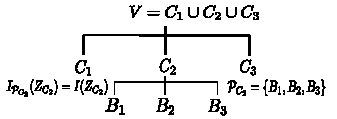
\includegraphics[width=\textwidth]{top_down.pdf}
      \caption{}\label{fig:top_down}
    \end{subfigure}~
  \begin{subfigure}[b]{0.29\linewidth}
    \centering
    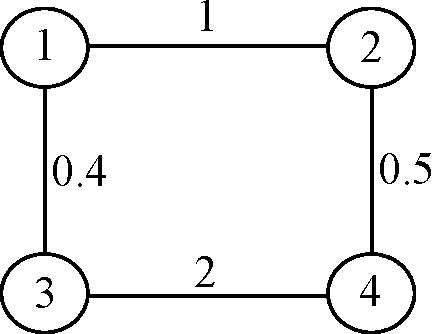
\includegraphics[width=0.8\textwidth]{threshold_b.pdf}
    \caption{}\label{fig:threshold_b}
  \end{subfigure}~
  \begin{subfigure}[b]{0.33\linewidth}
    \centering
    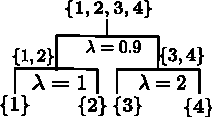
\includegraphics[width=\textwidth]{threshold_a.pdf}
    \caption{}\label{fig:threshold_a}
  \end{subfigure}
  \caption{聚类树示例}\label{fig:mmi_example}
  \end{figure}
自顶向下
获得聚类树的示意图由图 \ref{fig:top_down} 给出。
下面我们用一个简单的例子来说明聚类树的结构。
  \begin{example}\label{ex:mmi_tree}
考虑图 \ref{fig:threshold_b} 所示的情形,
$V=\{1,2,3,4\}$。互信息在图的边上标出,
比如 $I(Z_1;Z_2)=1, I(Z_1;Z_4)=0$。
利用定义 \ref{eq:IZV} 不难求出
$I(Z_V)=0.9$。 
我们可以写出完整的聚类结果:
\begin{equation*}
\P = 
\begin{cases}
\{\{1,2,3,4\}\} & \lambda < 0.9 \\
\{\{1,2\},\{3,4\}\} & 0.9 \leq \lambda < 1 \\
\{\{1\},\{2\},\{3,4\}\} & 1 \leq \lambda < 2\\
\{\{1\},\{2\},\{3\},\{4\}\} & \lambda \geq 2
\end{cases}
\end{equation*}
将各临界值标到聚类树上即得到如图
 \ref{fig:threshold_a} 所示的结果。
\end{example}
\subsection{HPSP算法}
在我们对PSP算法的改进中,仍将使用
算法 \ref{alg:psp} 中提到的
\texttt{DT} 子函数。
在算法 \ref{alg:psp} 中,我们观察到
每次调用 \texttt{DT} 的过程是相互独立的,
并没有利用到聚类树的 固有性质。
如果聚类树的嵌套性质被考虑进来的话,
我们可以在后面的计算中
仅在子图上进行 \texttt{DT} 的调用,
从而实现计算效率比PSP算法提升一个数量级。

在给出改进算法的描述之前,我们先定义两个对图的操作:
图限制(restriction)和图收缩(contraction)。
我们称把图$G$限制到集合$C\subseteq V$是指
考虑节点集为$C$而边的集合为$\{(i,j) \in E | i,j \in C \}$
的子图,
记为$G[C]$。给定$V$的分割 $\P=(C_1, \dots, C_k)$,
图根据$\P$收缩得到一个新的图,其节点集为
$[k]$,其中第$i$个节点对应$C_i$。边的集合为$\{(i,j) \in [k] | w(C_i, C_j) > 0 \}$。
其中$w(C_i, C_j)=\sum_{r \in C_i, s \in C_j} w_{rs} $
也是新图节点$i$和 $j$之间的权重。我们把收缩后的图记为
$G[\P]$。


在我们设计的算法中,
假设我们第一次调用 \texttt{DT} 后得到了
$\P_i = \{C_1, \dots, C_t\}$。
然后我们 分别对每个
$G[C_i](i=1,\dots, t)$
计算 PSP分割。
并从子图的计算中构造 $P_j(j>i)$。
对于 $\P_j(j<i)$,
我们对收缩后的图 $G[\P_i]$ 计算 PSP 分割
可以得到  $P_j(j<i)$ 的结果。
我们把如上的改进方法称为 HPSP (Hierarchical PSP),
其描述在算法 \ref{alg:psp_i_simplified} 中给出。

\begin{algorithm}[!ht]
	\caption{改进的求解主分割序列的算法(HPSP算法)}\label{alg:psp_i_simplified}
	\begin{algorithmic}[1]
		\REQUIRE 有向图 $G(V, E)$; 边的权值函数 $w(e)$,其中 $e\in E$
		\ENSURE 聚类树 $\mathcal{T}(K, E)$ 其中 $K \subseteq 2^{V}$ 表示节点集
    而 $E$ 表示边的集合。
		\STATE 初始化 树 $\mathcal{T}$:
     $V$ 是根节点,
     $\{j | j \in V\}$ 是诸叶节点,
     无其他节点。
		\STATE \texttt{Split}($G$)
		\FUNCTION{\texttt{Split}($G$)}
		\STATE $w$ 是 $G$ 所有边的权值之和。
		\STATE $\gamma' = \frac{w}{\abs{V(G)}-1}$
    其中 $V(G)$ 是 图$G$
    的节点集。
    \label{alg:gamma_apostrophe}
		\STATE $(\tilde{h}, \P')
    = \texttt{DT}(G, \gamma')$ 其中
    $\P'$ 是在 式 \eqref{eq:hlambda} 中达到
    最小值 $h(\gamma')$的分割
    并且 $\tilde{h}$ 是对应的最小值。 \label{line:DT}
		\IF{$\tilde{h} = - \gamma'$}
		\STATE 在聚类树
    $\mathcal{T}$ 中把权值 $\gamma'$ 标记在从 $V(G)$ 出发
    到其所有子节点的边上。
		\ELSE
		\FOR{$S$ in $P'$ and $\abs{S}>1$}
		\STATE 在聚类树
    $\mathcal{T}$ 中构造新的节点$s=S$,
    并修改 $S$中元素的父亲节点 为$s$,
    而$s$的父节点为$V(G)$。
		\STATE \texttt{Split}($G[S]$) \label{line:SplitDown}
    %其中 $\widetilde{G}[S]$ 是 $\widetilde{G}$ 限制在 $S$
    %上的子图。
		%\STATE 在 $\widetilde{G}$ 中将 $S$ 缩成一个节点。 % graph \widetilde{G} is modified
		\ENDFOR 
		\STATE \texttt{Split}($G[\P']$)		\label{line:SplitUp}
		\ENDIF
		\ENDFUNCTION
	\end{algorithmic}
\end{algorithm}

\begin{figure}[!ht]
	\centering
	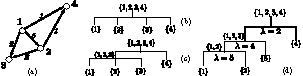
\includegraphics[width=10cm]{alg_illustration.pdf}
	\caption{HPSP 算法求解图(a)的主分割序列,聚类树经(b)、 (c) 演化到 (d) }\label{fig:alg_eg}
\end{figure}

\begin{example}
	我们用一个简单的例子来说明
  算法 \ref{alg:psp_i_simplified}。
  考虑图 $G(V, E)$,有 $V=\{1,2,3,4\}, E=\{(1,2),(1,3),(2,3),(1,4),(2,4)\}$。
  边的权值为 $w_{13}=2, w_{12}=5, w_{23}=2, w_{14}=1, w_{24}=1$。
	图 \ref{fig:alg_eg} (a)中画出了 $G$
  的结构。
  最初的聚类树结构如图 \ref{fig:alg_eg} (b)
  所示。
  根据 
  算法 \ref{alg:psp_i_simplified} 的
  第 \ref{alg:gamma_apostrophe} 行,
  我们计算出 $\gamma' = \frac{11}{4-1}, \tilde{h} = -\frac{16}{3} < -\gamma' $
  且 $\P' = \{\{1,2,3\},\{4\}\}$,
  于是我们得到如图 \ref{fig:alg_eg} (c)所示
  的聚类树结构。
	
	然后我们在 子图 $G[\{1,2,3\}]$ 上运用 PSP 算法,
  得到 $\gamma' = \frac{9}{2}, \tilde{h} = -5 < -\gamma'$
  并且 $\P= \{\{1,2\},\{3\}\}$。 
  后面的计算给出了聚类树剩余的边的权值,
  然后我们得到了最终的聚类树结构,如
  图 \ref{fig:alg_eg} (d)所示。
\end{example}	
\subsection{时间复杂度分析}

本小节我们分析上小节提出的 HPSP算法 (算法 \ref{alg:psp_i_simplified} )的时间复杂度。
首次说明一些惯用语,我们称图是稠密的,
如果它的边的数量是$n^2$的量级,
也即 $\abs{V} = n, \abs{E} = O(n^2)$。
对于稠密的图,由于最大流算法中需要多次遍历
边,会增大时间开销。一般PSP算法复杂度分析即针对最坏的情形,即稠密的图进行。
我们已知的结论有 \texttt{DT} 算法(算法 \ref{alg:psp} 第 \ref{alg:lambda_f} 行)
的时间复杂度是 $O(n^4)$, 而 PSP算法的 
时间复杂度是 $O(n^5)$ \citep{chan2017pin}。

我们使用 $T(n)$ 来代表 
\texttt{Split} 函数调用的
时间复杂度。
从算法 \ref{alg:psp_i_simplified} 中可知,
$T(n)$ 的递推关系式为
\begin{equation}\label{eq:Tn}
T(n) = \max \{ C n^4 + \sum_{i=1}^k T(n_i) +
T(k)\delta_{k<n} |
\sum_{i=1}^k n_i = n, n_i \in \mathbb{Z}_{+} \}
\end{equation}
在 式\eqref{eq:Tn} 中,
$Cn^4$ 代表 \texttt{DT} 的时间复杂度。
$\delta_{k<n} = 1$ 是 指示函数,当满足条件 $k<n$时取值为1,
否则 $\delta_{k<n}=0$。
针对 $T(n)$,我们有如下定理:
\begin{theorem}\label{thm:alg_complexity}
  在式 \eqref{eq:Tn} 中,若 $n_i \leq \frac{n}{2}$ 对于 $i=1,\dots,k$ 均成立,并且
   $ k \leq \frac{n}{2}$, 
   则 $T(n) = O(n^4)$。
\end{theorem}

定理 \ref{thm:alg_complexity} 所要求的条件
限制了聚类树的结构。
该定理指出,若对于每个非叶节点,其后代数都不超过 $\frac{n}{2}$,则HPSP
算法的时间复杂度是  $O(n^4)$。
该条件适用于很多情形下的聚类树,
即使有个别节点不满足其假设,$T(n) = O(n^4)$也成立。
因此,定理 \ref{thm:alg_complexity} 表明,我们在保证有相同计算结果的前提下,
提出的HPSP 的时间复杂度的结果要比
PSP算法 \ref{alg:psp} 的$O(n^5)$ 的结果快一个数量级。

在定理 \ref{thm:alg_complexity} 的条件不满足时,
考虑最坏的情况,也即聚类树的深度达到了 $O(n)$ 的数量级,
则 \texttt{DT} 不可避免地要调 用 $O(n)$ 次。
在这种情形下,
$T(n)$ 的复杂度的上界是 $C(3^4+4^4 + \dots + n^4) \sim \frac{1}{5}Cn^5$,
仍比 算法 \ref{alg:psp} 的结果
快 $5$ 倍。
\subsection{聚类树的数据结构}
在层次聚类中一般使用关联矩阵(linkage matrix)构造聚类树
\cite{D2011Modern},但这种方法
仅限于一次聚合两个节点的场景。
在允许一次聚合多个节点的情形下,可以使用带权的并查集(weighted Union-Find set)的方法自底
向上构造聚类树
\cite{chan2020agglomerative}。 
但由于我们设计的HPSP算法是
自底向上和自顶向下的混合,不能照搬关联矩阵和并查集的数据结构,而是要结合
HPSP算法 \ref{alg:psp_i_simplified} 的特点重新设计。
为此,
我们采用选取代表元素的方法来构造聚类树,比如对于
聚类树的中间节点$\{1,2\}$选取较小的元素1来代表。
这样做的一大优势是无需为中间节点额外开辟空间,降低算法的空间复杂度。
具体而言,我们采用父节点数组$K$来储存树的结构,而和聚类树边权重相关的数据
用另一数组$W$储存。聚类树的空间复杂度为$2|V|$。
基于以上数据结构,
HPSP算法 \ref{alg:psp_i_simplified} 使用静态数组的实现
如算法 \ref{alg:psp_i_simplified_tree_array} 所示。

\begin{algorithm}[!ht]
	\caption{从有向图获取聚类树}\label{alg:psp_i_simplified_tree_array}
	\begin{algorithmic}[1]
		\REQUIRE 有向图 $G(V, E)$; $V=[n]$,边的权值函数 $w(e)$,其中 $e\in E$
		\ENSURE 聚类树 $\mathcal{T}=(K, W)$, $K,W$ 为$n$长的数组,
    $K[i]$ 表示树中节点$i$的父节点的ID,
    $W[i]$表示节点$i$到其父节点的权值。
		\STATE 初始化 $n$ 长的数组 $\mathcal{T}$
     和$W$。
		\STATE \texttt{Split}($G, 1$)
		\FUNCTION{\texttt{Split}($G, s$)}
		\STATE $w$ 是 $G$ 所有边的权值之和。
		\STATE $\gamma' = \frac{w}{\abs{V(G)}-1}$
    其中 $V(G)$ 是 图$G$
    的节点集。
		\STATE $(\tilde{h}, \P')
    = \texttt{DT}(G, \gamma')$ 
		\IF{$\tilde{h} = - \gamma'$}
		\STATE $W[i]=\gamma'$ for $ i \in V(G)$
    \STATE $K[i]=s$ for $i\in V(G)$
    \ELSE
		\FOR{$S$ in $P'$ and $\abs{S}>1$}
		\STATE \texttt{Split}($G[S], j$),其中$j$为$S$中最小的元素。
		\STATE $G=$ \texttt{Contract}($G, S, j$) \label{alg:contract}
    \ENDFOR 
		\STATE \texttt{Split}($G, s$)
		\ENDIF
		\ENDFUNCTION
	\end{algorithmic}
\end{algorithm}

为标记聚类树中每个节点的父节点,
我们在算法 \ref{alg:psp_i_simplified_tree_array} 的 \texttt{Split} 函数中增加了
一个参数$s$,$s$是当前所操作的图中所有节点序号最小的,
对应到聚类树中这些节点的父节点ID。

在第 \ref{alg:contract} 行的\texttt{contract}函数 是在图$G$中
将$S$中的各节点缩为一个点$j$,边的权值也做相应的调整。
为了提升算法运行效率,和图限制$G[S]$类似,我们可以避免构建新图的操作,
而是直接在原图$G$上进行修改。

另外,从构造好的聚类树中获取正确的分割也是
我们要考虑的问题。
\citet{chan2020agglomerative}曾采用一种
类似深度优先搜索的策略在聚合的过程中逐步获取分割。
由于我们未存储子节点的信息,因此我们在
获取分割的实现策略上需要另辟蹊径。
为此,我们采用自底向上的方法获取全部的分割,
具体实现见算法 \ref{alg:get_psp}。

\begin{algorithm}[!ht]
	\caption{从聚类树获取主分割序列}\label{alg:get_psp}
	\begin{algorithmic}[1]
		\REQUIRE 聚类树 $\mathcal{T}=(K, W)$
		\ENSURE 序列 $L=[\lambda_1, \dots, \lambda_k]$
    和 $\mathcal{Q}=[\P_0, \dots, \P_k]$。
    \STATE 初始化 $Q\leftarrow \{ \{\{i\}|i\in [n]\} \}, C\leftarrow [n]$
    与哈希字典 $D$,$D$把不存在的键值映射到空集。
    \WHILE{$|C|>1$}
		\STATE $(\P,\gamma, C)$ \leftarrow \texttt{Merge}($C$)
    \STATE 将 $P$ 加到 $Q$ 的头部,并将 $\gamma$ 加到 $L$ 的头部。
    \ENDWHILE
		\FUNCTION{\texttt{Merge}($C$)}
    \STATE $\gamma = \max_{i\in C} W[i]$
    \STATE $D[k] = \{ j\in C | K[j] = k, W[j]=\gamma\} \cup \{k\} \cup D[k]$
    \FOR{$ j \in D[k]$}
    \STATE $D[k] \leftarrow D[j] \cup D[k]$, 并从$D$中删除键值$j$。
    \ENDFOR
    \STATE $C' \leftarrow  \{j\in C | W[j]<\gamma\}$
    \STATE $\P=\{D[k] | k \in \texttt{key}(D)\} \cup \{\{i\} | i \in [n]\backslash \cup_{k \in \texttt{key}(D)} D[k] \}$
    \RETURN $(\P, \gamma, C')$
		\ENDFUNCTION
	\end{algorithmic}
\end{algorithm}

在算法 \ref{alg:get_psp} 中,我们
使用了额外的数组$C$来表示合并后当前
剩余的节点,字典$D$储存了如何把剩余的节点展开成聚类簇
的信息。由于 \texttt{Merge} 函数最坏调用$n$次,
而计算$\gamma$的时间复杂度是$O(n)$,其它操作不超过$O(n)$,
因此整个转换算法的时间复杂度是$O(n^2)$,相比
定理 \ref{thm:alg_complexity} 中
给出的HPHP 的$O(n^4)$的时间复杂度,转换本身的时间开销
可忽略不计。

\subsection{代码实现}
尽管最大流算法包比较多,但我们尚未发现
求解层次分割(式\eqref{eq:PSP_structure})的开源实现。
因此我们使用 C++ 实现了跨平台的PSP算法 \ref{alg:psp} 
(内嵌 \texttt{DT} 算法),并且
我们提供了Python编程语言的接口函数,并在 \url{pypi.org}
平台上以 pspartition
的名字发布,以供后面的研究者使用。
我们的实现使用 CMake 编译,依赖于第三方库 LEMON \cite{dezsHo2011lemon}。 
LEMON 库在我们的算法包中用于构建所需的图数据结构和最大流算法。
这里顺便提及的一点是 LEMON 库里使用的
最大流算法是基于最大标签选择策略的前置推送-标签重贴算法。
根据文献\inlinecite{ahuja1997computational}的比较,该算法
的效率相比其他求解最大流问题的算法有明显的优势。

在Python的接口函数方面,我们采用了CPython
跨语言编程的方式,将由 NetworkX \cite{SciPyProceedings_11} 构建的图
转换成用边表示的图传递到C++中的类构造函数中,
计算完成后再把C++中的集合转换成Python中的列表
进行返回。用于求解例 \ref{ex:psp} 的示例 Python 代码如下。
\begin{lstlisting}[language=Python]
  from pspartition import PsPartition
  a = [[0,1,1], [0,2,5], [1,2,1]] #graph edge list,(i,j,weight)
  p = PsPartition(3, a) #3 nodes
  p.run()
  cv = p.get_critical_values() #[2,5]
  pl = p.get_partitions()#[[{0,1,2}],[{0,2},{1}],[{0},{1},{2}]]
\end{lstlisting}

\subsection{求解主分割序列算法效率比较}
在本节中,我们将比较 HPSP 算法和PSP算法
(算法 \ref{alg:psp} )
以及基于参数最大流改进方法\cite{kolmogorov}
的运行效率。我们使用两种不同的数据集,图的边具有不同的
稠密程度。

第一个数据集是由
4个相同大小的高斯斑点(Gaussian Blobs)组成,但我们可以改变
每部分的样本数量。我们使用式
  $w_{ij}=\exp(-\eta ||x_i-x_j||^2)$
计算图中边的权值,边的数量满足 $|E|=\Theta(|V|^2)$。
这里$\Theta$表示$|E|$与$|V|^2$量阶相同。
\newglossaryentry{not:fntheta}
{
  type=notation,
  name={$f(n)=\Theta(g(n))$},
  description={当$n\to \infty$时,$f(n)$和$g(n)$ 具有相同的量阶}
}
第二个数据集由两层随机块组成,
边的数量满足 $|E|=\Theta(|V|^{\frac{3}{2}})$。

我们使用CPU时间来衡量算法的时间复杂度。
通过改变节点的数量,
我们可以得到如图 \ref{fig:esc} 所示的实验结果,
对于高斯斑点数据,在节点数为$400\sim 500$时,
我们的实现比之前最优的算法要快100倍以上。
而对于两层的随机块数据,在节点数为1296时,
算法效率提升了约70倍。
\begin{figure}
	\centering
	\begin{subfigure}{0.45\textwidth}
		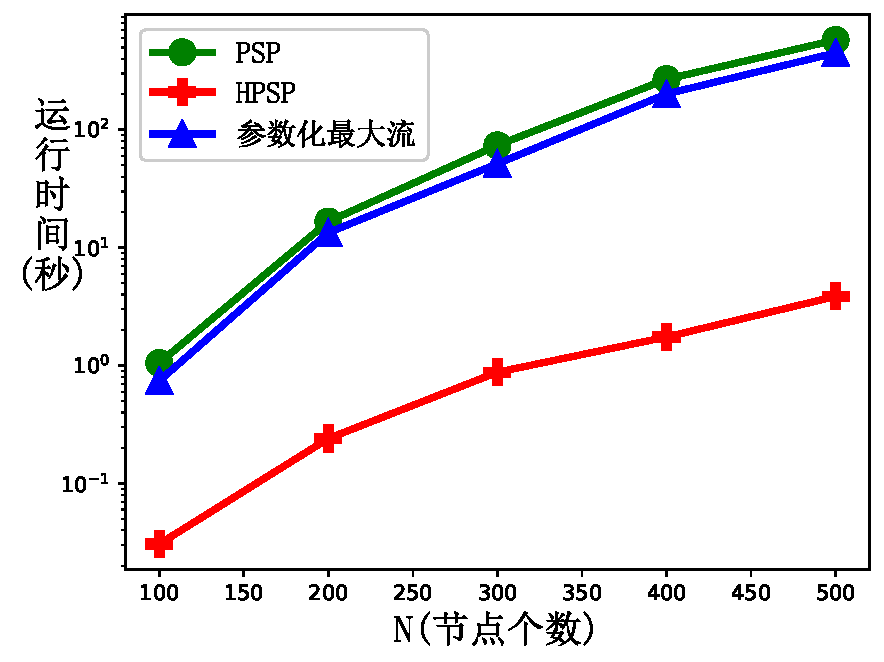
\includegraphics[width=\textwidth]{2019-08-26-gaussian.pdf}
    \caption{高斯斑点x4}
	\end{subfigure}
	\begin{subfigure}{0.45\textwidth}
		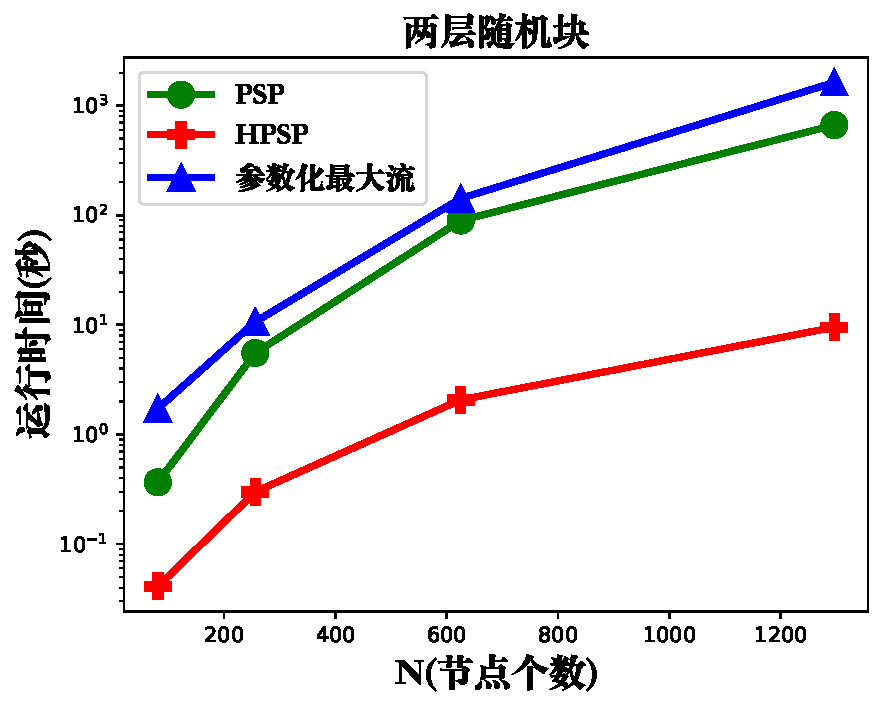
\includegraphics[width=\textwidth]{2019-09-19-two_level.pdf}
    \caption{两层的随机块}
	\end{subfigure}
	\caption{
  不同PSP实现的速度比较}\label{fig:esc}
\end{figure}

另外我们注意到,
基于参数化最大流的
算法\citep{kolmogorov}虽然在理论分析中复杂度
比 PSP算法快一个数量级,但在实践中表现不佳。
这可能与计算过程中构造中间图的结构
和维护并发线程的额外成本有关。在实际实现中,
并发线程的创建和销毁的时间开销是不可忽略的,而这一部分
在复杂度理论分析中并未考虑。
另外,\citet{chan2020agglomerative} 提出的基于 最小化范数底的聚合算法
也能用于求解图上的主分割序列,但由于该方法是针对一般的
随机变量聚类问题提出的,对熵函数求值的额外开销过大,
也面临理论优美、实际效率不高的问题。
%但该方法利用了某种并行化的方法,以及受到数值精度的影响,,但在实际算法中难以实现。

\section{实验结果}\label{sec:hierarchical_experiment}
\subsection{社团的层次化发现}
\label{subsec:cd}
尽管在发现社团的单层结构方面
有很多算法取得了成功,自动发现
复杂网络中的社团层次结构仍是一个困难的问题。
在本节中,我们通过实验来证明PSP算法
在恰当定义“边的权重”后,可以成功恢复两层图的层次结构。

对于一个无权图,如果我们简单地把
所有边的权值赋成1,
我们只能得到平凡的聚类树,也即聚类树
只有根节点和叶节点。这个论断可以从如下
定理中得到:
\begin{theorem}\label{thm:triangle}
  在图$G$中,对于没有边相连的两个节点 $w_{ij}=0$。
  并且对于任意三元组$i,j,k \in V$ 权值满足三角不等式 
  $w_{ij} + w_{jk} \geq w_{ki}$,
  则该图的聚类树是平凡的。
\end{theorem}
  
我们通过实验发现使用下述的方法对无权图进行重新
赋权可以达到较理想的效果:
\begin{equation}\label{eq:wij_scheme}
    w_{ij} = 1 + \abs{\{k | (i,k),(j,k) \in E \}} \textrm{ for } (i,j) \in E
\end{equation}
式 \eqref{eq:wij_scheme} 对$w_{ij}$
的赋权方法是计算从$i$到$j$不超过两跳的路径数量。

下面我们在一个具有两层结构的图上验证我们的
赋权方法。该数据集在文献
\cite{arenas2006synchronization} 中用于
研究基于Kuramoto 模型的社团层次发现算法,
其结构如图 \ref{fig:c1} 所示,
一共有 $256$ 个节点。

\begin{figure}
	\centering
	\begin{subfigure}{0.45\textwidth}
		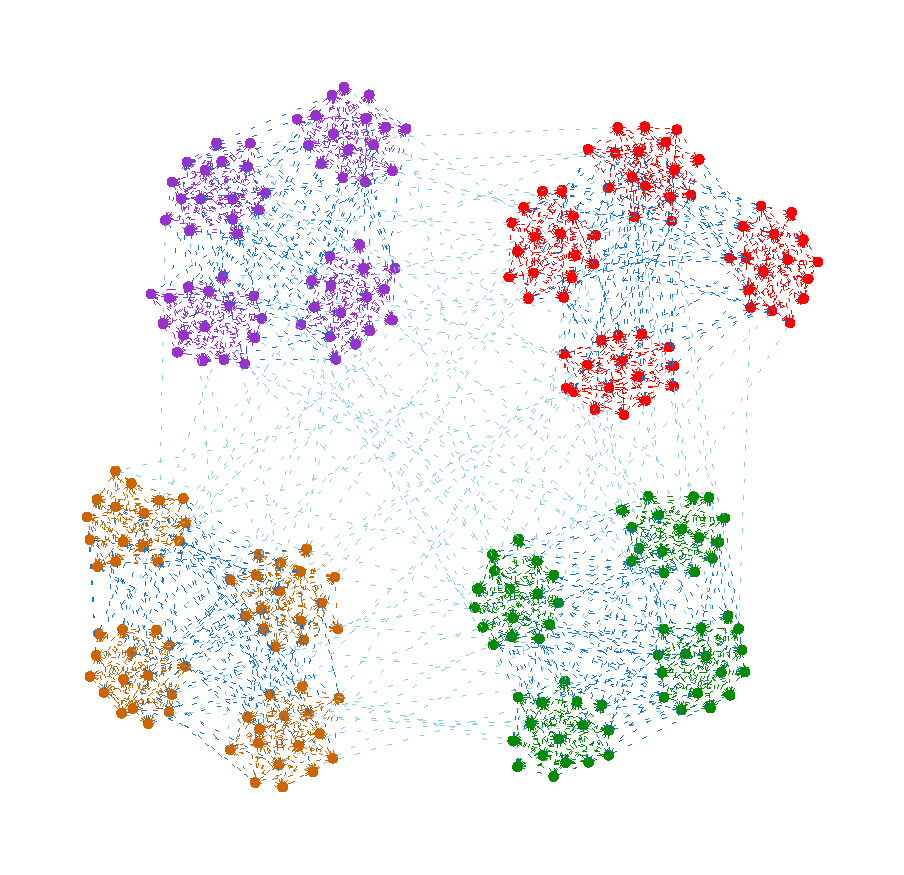
\includegraphics[width=\textwidth]{two_level-2023-02-16.pdf}
		\caption{拓扑结构,参数取值为$z_{\mathrm{in}_1} = 14, z_{\mathrm{in}_2} = 3, z_{\mathrm{out}}=1$。}\label{fig:c1}
	\end{subfigure}
	\begin{subfigure}{0.45\textwidth}
		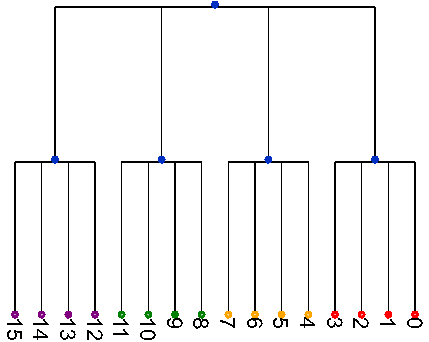
\includegraphics[width=\textwidth]{tree_info-clustering.pdf}
		\caption{聚类树结构,可用PSP算法完全恢复出来。每个叶节点仍包含16个子节点未画出。}
    \label{fig:c2}
	\end{subfigure}
	\caption{具有两层结构的图示意}
\end{figure}

该两层结构的图在宏观层面它包含有 4个 社团,
而每一个中等规模的社团在微观层面又包含4个小社团,
每个小社团有16个节点。
我们用 $z_{\mathrm{in}_1}$ 表示
在小社团内部每个节点连接的边的平均数量;
用 $z_{\mathrm{in}_2}$ 表示
每个大社团内部的中等规模社团之间相互连接的边的平均数量;
用 $z_{\mathrm{out}}$ 表示
不同大社团之间相互连接的边的平均数量。
通过变化参数设定
$\{z_{\mathrm{in}_1}, z_{\mathrm{in}_2}, z_{\mathrm{out}} \}$,
我们能得到不同疏密程度的图。

为比较通过算法推断出的聚类树的结构和真实聚类树的区别,
我们使用 归一化的 Robinson-Foulds 距离度量\cite{ROBINSON1981131}。
它描述了两个具有不同拓扑结构的树之间的距离,
其取值在$[0,1]$ 之间。
我们将HPSP算法与
格文-纽曼算法\cite{girvan2002community}
和 BHCD (贝叶斯层次聚类算法\cite{blundell2013bhcd})进行比较,
比较的结果如图 \ref{fig:cdr} 所示。
从图 \ref{fig:cdr} 中可以看到,在三种不同的参数配置下,
HPSP算法相比其他方法 可以获得
与真实聚类树更相似的层次结构。

\begin{figure}
	\centering
	\begin{subfigure}{0.33\textwidth}
		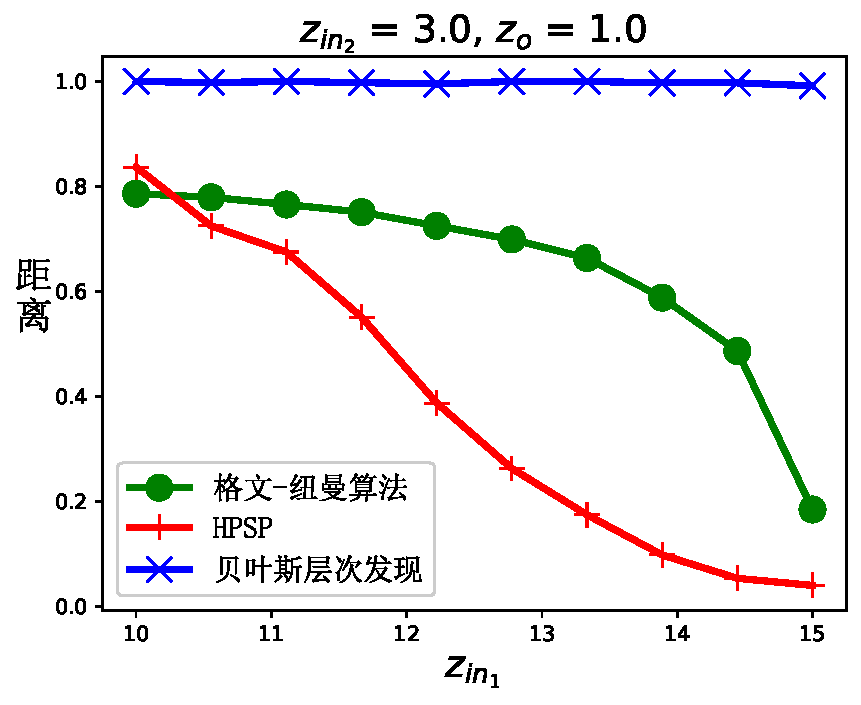
\includegraphics[width=\textwidth]{z_in_1.pdf}
		\caption{}
	\end{subfigure}~
	\begin{subfigure}{0.33\textwidth}
		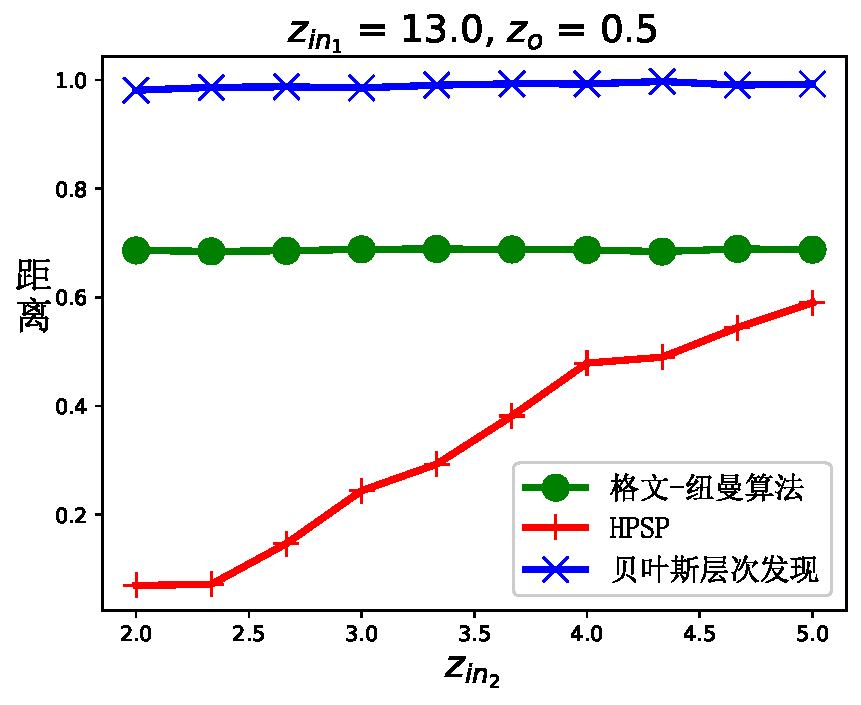
\includegraphics[width=\textwidth]{z_in_2.pdf}
		\caption{}
	\end{subfigure}~
	\begin{subfigure}{0.33\textwidth}
		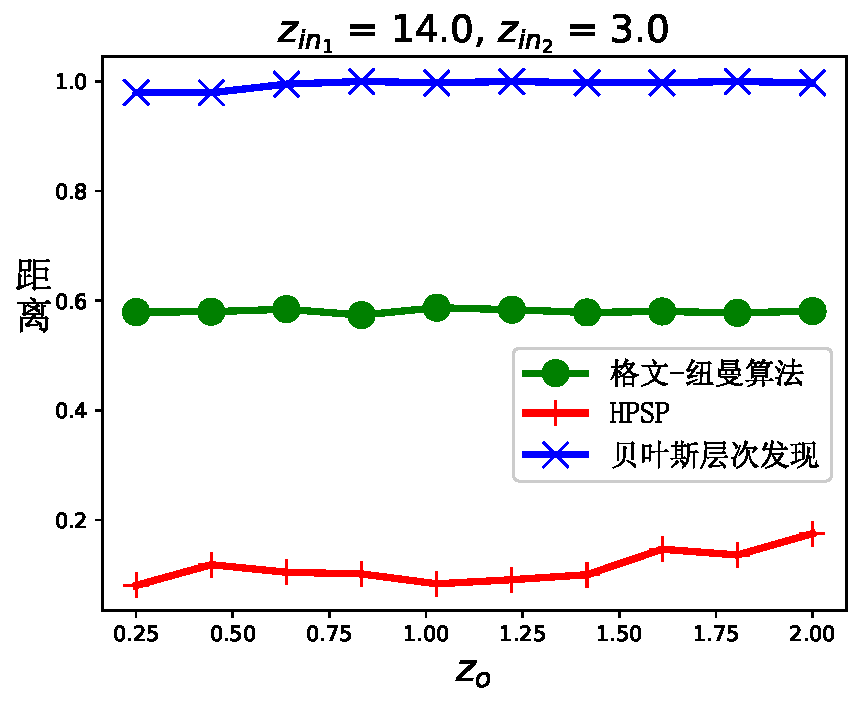
\includegraphics[width=\textwidth]{z_o.pdf}
		\caption{}
	\end{subfigure}
	\caption{不同社团层次化发现算法的性能比较。
  更小的距离意味着与真实的聚类树更相似的结构。
  }\label{fig:cdr}	
\end{figure}

\subsection{数据聚类}
\label{sec:data_clustering}
社团发现是输入一张图获得节点所属的类别,而
数据聚类的任务与社团发现相同,但其输入是一个数据矩阵,
其中行数是数据的个数而
每一行的向量代表该数据的特征。二者可以通过
输入数据的格式转换来实现算法互通。一般而言,
从数据矩阵到图的变换是可以通过选取一
相似度度量$d(\cdot,\cdot)$作用到数据上
获得图中边的权值,即$w_{ij}=d(x_i, x_j)$。
在这一节中,
我们研究的重点是如何用
HPSP算法 实现数据的聚类的任务。
已有学者用RBF核作为相似度度量,
基于类似PSP的算法进行非层次聚类的
尝试\cite{mac},而本节主要
针对HPSP算法在层次聚类问题上进行实验。

为了比较不同的层次聚类方法,最好直接比较聚类树。
为此,
我们使用来自\citet{khan2001classification}的基因表达的数据集。
该数据集共有6000多条基因数据,训练集的特征维度是64,
测试集是25。这里我们只使用前300条基因的数据。
由于我们不知道数据的真实聚类树的结构,
我们采用分割特征的方法,
分别在两个具有部分特征的数据集上应用聚类算法,
并比较得到的聚类树的相似程度。
这样做的另一个好处是我们还可以测试每种聚类方法的稳定性。

我们将HPSP算法与基于平均距离度量的系统聚类法、
贝叶斯玫瑰树算法
\cite{blundell2011discovering}
进行了比较。
树的相似性度量是未归一化的 Robinson-Foulds 距离,
它是将一棵树转换为另一棵树的步骤数
(一个步骤指添加或删除一条边)
\citep{day1985optimal}。
针对不同样本数量的实验
结果如图 \ref{fig:shc} 所示。
从中可以看出,对于经典的系统聚类方法,
其在不同特征子空间的树的结构相差最大,稳定性较差。
当$n$较大时,HPSP算法和贝叶斯玫瑰算法稳定性相当。
但当$n$较小时,HPSP算法表现最好,距离相比贝叶斯玫瑰算法减小了约30\%。

\begin{figure}[!ht]
\centering
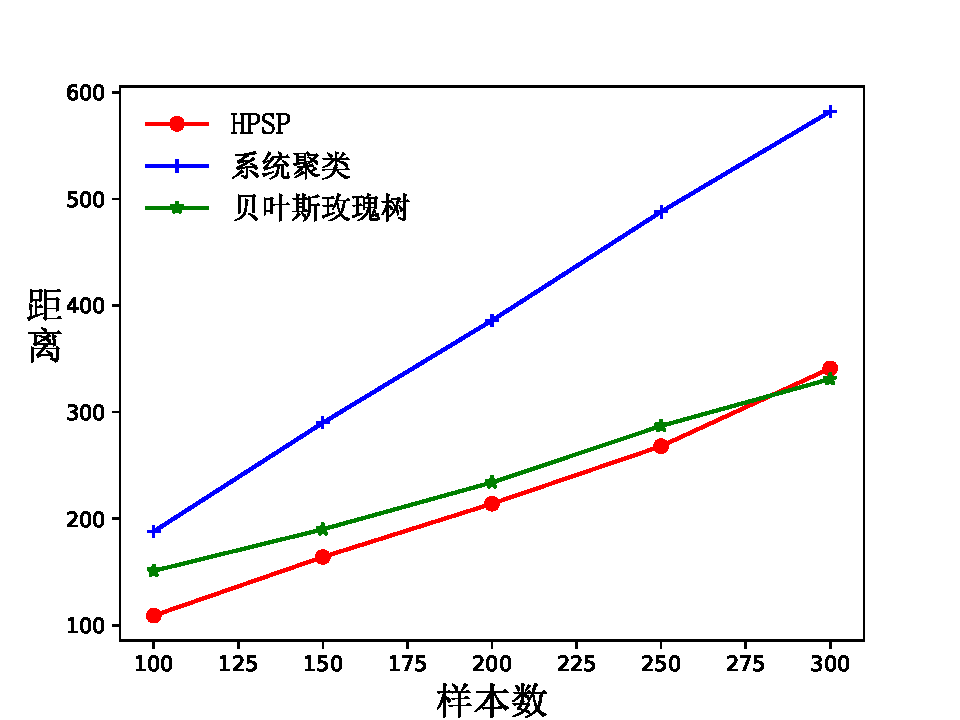
\includegraphics[width=8cm]{genes.pdf}
\caption{不同层次聚类算法稳定性的比较}\label{fig:shc}
\end{figure}

为展示我们提出的HPSP算法在实际问题中的应用效果,我们考虑一个简单的例子——自然语言的层次聚类问题。
一方面我们通过该实例展示HPSP算法在社团发现实际数据上的应用效果,
另一方面,考虑到语言的分类领域对印欧语言研究较多,已有完善的标准;
而对其他地区方言和少数民族语言研究较少,使用
算法自动聚类对于语言分类的研究有所裨益 \cite{nasution2019visualizing}。

我们使用的数据是关于词汇相似率的数据。
词汇相似率是一个百分比,表示两种语言中有相同词意和书写方式的词汇比例
\cite{bella2021database}。
我们从Bella提供的数据中选取了世界66种常用语言,选取的标准是原
数据集中词汇相似率置信程度高且两两间均有相似率的语言。
在我们选取的66种语言中,其中一种人造语言(世界语),
两种古典语言(梵语、拉丁语),其余均为现代语言。
在此基础上我们用 HPSP 算法进行聚类,得到了如图 \ref{fig:language_tree} 所示的聚类树。

\begin{figure}[!ht]
    \centering
    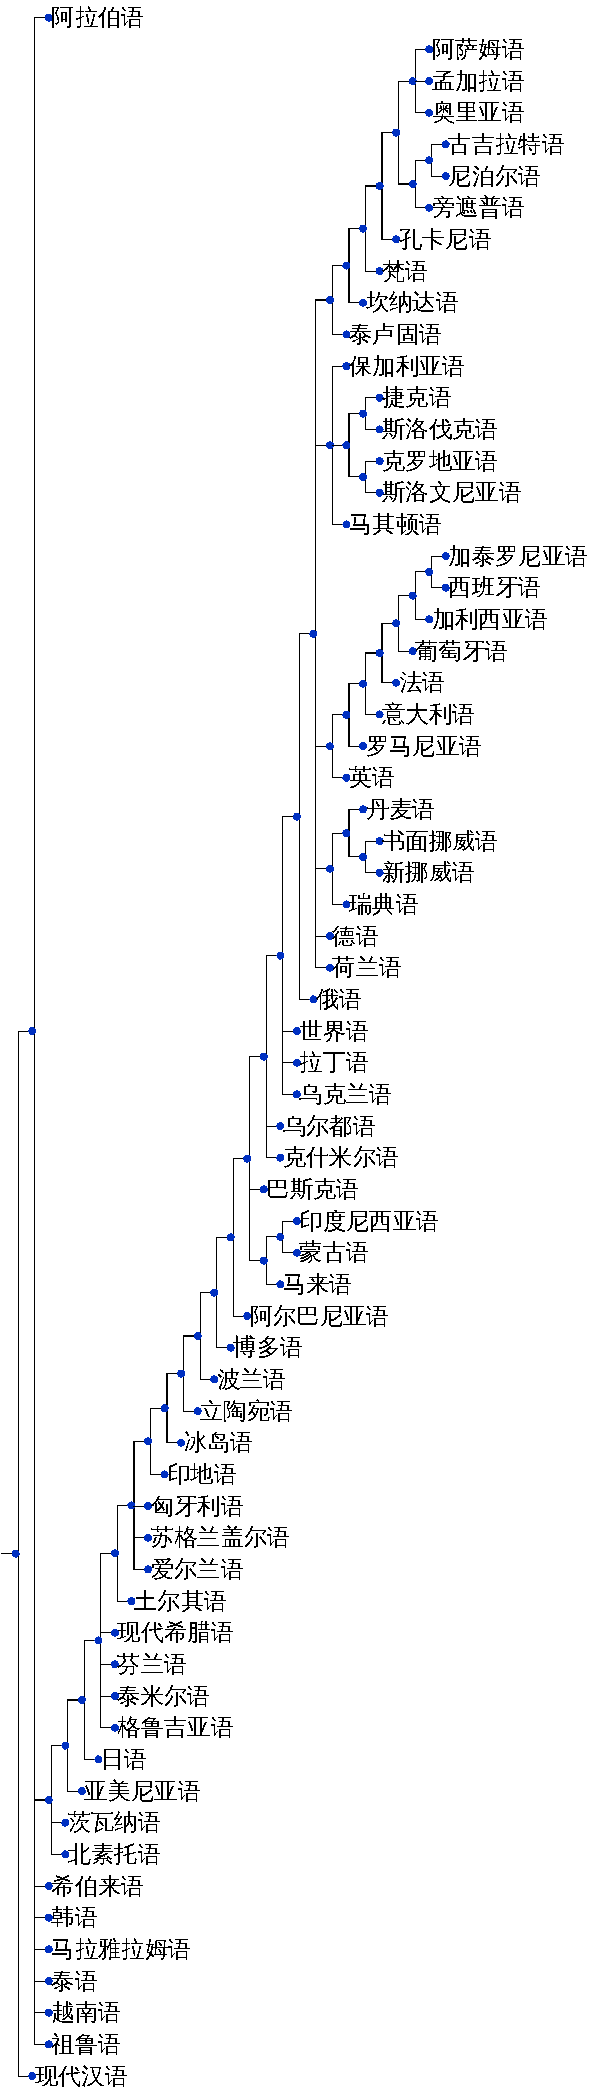
\includegraphics[height=0.9\textheight]{language_tree.pdf}
    \caption{使用HPSP算法获得的世界常用语言聚类树示意图}\label{fig:language_tree}
\end{figure}

从图中我们可以解读出一些与比较语言学相一致的结论。
首先上图包含了一些在同一国家不同地区使用的语言(西班牙、印度、南非),它们在聚类树中位置较近。
比如西班牙语、加泰罗尼亚语和加利西亚语同属于西班牙,在聚类树中距离很近。
其次从语言进化的角度,具有相同祖先的语言在聚类树中位置较近。比如法语、西班牙语、葡萄牙语、意大利语、
罗马尼亚语同由拉丁语演变而来,
图 \ref{fig:language_tree} 中亦反映出来这五种语言距离很近。

有学者用了普通的聚合聚类的方式对10种常用语言进行聚类 \cite{al2017characterization}。
我们在这里指出其结果存在一定的不足,比如荷兰语和德语同属于日尔曼语系,在
其获得的聚类树中无法体现,而在我们得到的图中荷兰语和德语的亲近性一目了然。

尽管用算法自动生成的语言聚类树相比语言学家给出的语言进化树仍面临缺少
可解释性和某些方面的准确性,但该方法易拓展到非印欧语系的研究,
为印欧语言和非印欧语言的比较提供了参考。比如从我们的图中可以看到
现代汉语、日语、英语三者的相似度大小,尽管三种语言是属于不同的语系。



\section{HPSP算法在异常值检测领域的应用}\label{sec:outlier}
异常值检测是对异常数据(称为异常值点)的识别,
这些异常数据不同于其他多数数据(称为正常值点)
\citep{grubbs1969procedures}。
在本节中,我们考虑将HPSP算法用到异常值检测领域。

首先我们在理论层面探讨异常值检测背景下HPSP算法的应用。
假设一个简单的情形,所有正常值点属于同一类别,
并且集合$B$达到式\eqref{eq:largest_threshold}中的
最大值,
我们认为$B$中的元素是正常值点,而$V\backslash B$ 是异常值点。

我们进一步考虑,假设有一个新的点$i'$加入到
现有的图 $G$ 中,如何判断它是正常值点还是异常值点。 
事实上,对于加入$i'$的图来说,
我们可以用HPSP算法计算一个新的最大临界值
$\gamma'_N$,
并把它与 $\gamma_N$作比较。 由式\eqref{eq:largest_threshold}易得
$\gamma'_N \geq \gamma_N$。如果不等号严格成立,我们看到$i'$的作用是使得
多变量互信息的最大值增大了,说明$i'$与图$G$结合得更紧密,是正常值点,否则为异常值点。
实际上,我们不需要重新计算$\gamma'_N$就可以做出相同的判断,这个理论保证由下面的
定理给出。
\begin{theorem}\label{thm:main_N}
  假设 $B$ 关于图$G$ 达到式\eqref{eq:largest_threshold}中的
  最大值,$\gamma_N, \gamma'_N$ 分别是图$G$加入新的点$i'$前后的最大临界值,则有
\begin{equation}
\gamma'_N > \gamma_N \iff  \sum_{i \in B} w_{ii'} > \gamma_N 
\end{equation}
\end{theorem}
定理 \ref{thm:main_N} 给出了一种划分正常值点边界的方法,
假设图$G$的第$i$个点
对应一个高维空间的向量$x_i$,新加入的点对应的向量是$x$,
边的权值由RBF核给出,参数为$\eta$,则检测边界的方程为:
\begin{equation}\label{eq:sum_exp_gamma_N}
  \sum_{j \in B} \exp(-\eta \norm{x - x_j}^2)= \gamma_N
\end{equation}

上述讨论假设了所有正常值点同属一个类别,
在实际应用中可能具有局限性。
下面我们考虑在多分类问题中存在若干异常值点时的检测策略。
我们的目标是获得数据的一个分割,其形式为
$\{C_1, \dots, C_K, \{x_1\}, \dots, \{x_M\}\}$。
这里 $K$ 表示类别数 而 $M$ 表示异常值点的个数。
这两个参数在实际问题中通常是未知的,
我们基于 HPSP 算法来获得$K, M$的值,并同时给出聚类和
异常值检测的结果。

如果 $K$ 和 $M$ 较小, 使用式 \eqref{eq:PSP_structure}
的记法, 处理这种情况的一种经验性但合理的方法是从
$\{\P_k, \P_{k-1}, \dots, \P_0\}$中找到一个划分
$\P_{k-r}$,使得$K,M$都比较小。
对于此多目标优化问题,我们需要一个折中方案,即通过枚举
$r=1,2,\dots$ 求解下面的优化问题:
\begin{align}\label{eq:outlier_detection_proposal}
& \min_{r\in Z^+} r \\
\textrm{s.t.}\, & f(r):=(r+1)\abs{\P_{k-r}} < n \notag
\end{align}
在式\eqref{eq:outlier_detection_proposal}中,我们注意到函数
$f(0)=|\P_k|=n$ 和 $f(k)=k+1<n$ ,从而可知优化问题有解。

然后我们用 $\P_{k-r}$ 中元素个数大于1的集合来标记各类别中的正常值点,
元素个数小于1的集合为异常值点的集合。

如果需要预测新的观测值是否是异常值点,
我们使用类似于式\eqref{eq:sum_exp_gamma_N}给出的边界方程判决规则。
假设 $\lambda_{k-r}$ 是$\P_{k-r}, \P_{k-r+1}$ 两个分割对应的
分界值并且图$G$边的权值是使用 RBF 核 来构建的,
那么边界曲线方程可以写成下面的形式:
\begin{equation}\label{eq:boundary_curve_multiple}
\sum_{j \in C_i} \exp(-\lambda \norm{x - x_j}^2)= \lambda_{k-r}, \textrm{ 其中 } \, C_i \in \P_{k-r} \textrm{且}\,  \abs{C_i} > 1
\end{equation}
注意到 $C_i$ 是其中一个类别,
并且 一共有 $K$ 个 边界曲线。
如果新的观测值落在所有这些边界曲线的外部,
那么我们将其归类为异常值点。


我们准备了三个人工数据集来验证我们提出的异常值检测算法。
第一个数据集是一个高斯斑点,
其中有一些噪声点均匀分布在一个正方形中。
第二个数据集是我们将 $(0,0)$ 这个点加入
到 \ref{sec:data_clustering} 节所描述的有4个类别的
高斯斑点里。
最后一个数据集是两个错开的半月形状,
并且其周围分布着一些
噪点。
构造相似图的权值我们采用 RBF 核,其 异常值检测
效果如图 \ref{fig:boundary} 所示。
从前三幅图可以看出,由式\eqref{eq:boundary_curve_multiple}
给出的边界曲线近似于正常值点的闭包曲线。
\begin{figure}[!ht]
	\centering
	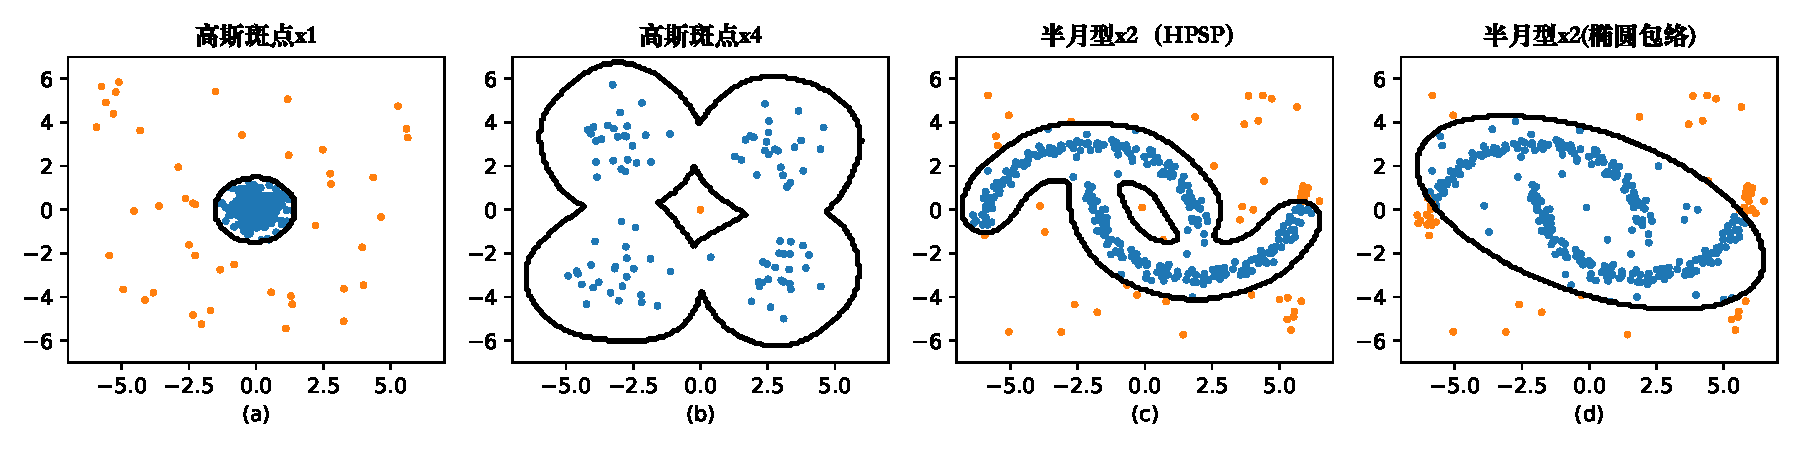
\includegraphics[width=\textwidth]{outlier_boundary_illustration.pdf}
	\caption{在人工生成的数据集上
  检测边界的形状}
  \label{fig:boundary}
\end{figure}

另外我们也
在图 \ref{fig:boundary} (d)画出了椭圆包络\cite{rousseeuw1999fast}(elliptic envelope)方法的决策边界曲线。
由于后一种方法假设内部数据分布在凸的区域,
因此决策边界是椭圆形状,
不能很好地反映真实数据的分布。

下面我们针对不同的数据集比较本节提出的异常值检测方法和其他常用的
异常值检测算法的性能。
我们使用 5 个数据集: 高斯斑点、 半月型、Lymphography
\cite{lazarevic2005feature}、 Glass 和 Ionosphere \cite{keller2012hics}。 
前两个数据集如前所述是
人工生成的,
而后三个数据集在异常值检测算法比较的文章中大量使用
\cite{campos2016evaluation}。
我们对比的方法包括
局部异常因子(local outlier factor \citep{Breunig})、
孤立森林(isolation forest \citep{if})、
椭圆包络  和
一类支持向量机 (one class SVM \citep{svm})。 
我们使用TPR和TNR来衡量检测的整体性能。
%正常值点被视为正样本。
TPR衡量的是正常值点集合中正确检测的百分比,
而TNR衡量的是异常值点中正确检测的百分比。
通常而言,一种检测方法很难在这两个指标上都获得高分。
我们设法最大化TNR,同时控制每种方法的TPR$\geq 90\%$。
每个方法的超参数和相似度度量都经过了调优,
TNR的最佳结果如表 \ref{tab:odm} 所示。我们可以看到,
基于HPSP算法的异常值检测(信息检测)在 GaussianBlob、Moon 和
Lymphography 数据集上表现最好,与局部异常因子效果差不多,
但在 Glass 和  Ionosphere 两个数据集上性能有待提升。
\begin{table}
  \begin{adjustbox}{width=\columnwidth,center}
\begin{tabular}{cccccc}
  \hline
         TPR/TNR        &  高斯斑点   &      半月型       &  Lymphography  &     Glass     &  Ionosphere   \\
  \hline
      信息检测    & 100\%/100\% & 97.4\%/100\%  & 97.9\%/100\% & 91.2\%/11.1\% & 90.7\%/48.4\% \\
      局部异常因子 & 100\%/100\% & 100\%/100\% & 98.6\%/83.3\%  & 96.6\%/22.2\% & 90.2\%/82.5\% \\
   孤立森林   & 100\%/100\% &  96.7\%/77.8\%  & 99.3\%/100\% & 89.8\%/11.1\% & 80.4\%/65.1\% \\
    椭圆包络   & 100\%/100\% &  91.3\%/42.2\%  & 93.0\%/83.3\%  & 94.6\%/0.0\%  & 93.3\%/88.1\% \\
     一类支持向量机     &  98.8\%/91.1\%  &  93.0\%/55.6\%  & 93.0\%/66.7\%  & 91.7\%/22.2\% & 83.1\%/69.0\% \\
  \hline
  \end{tabular}
\end{adjustbox}
\caption{不同异常值检测算法的比较}\label{tab:odm}
\end{table}

在上面的实验中我们假定已知异常值点的数量,
而实际上我们本节提出的方法只需给出权值$\eta$即可自动获取类别数和异常值点的数量,
相比其他需要提前知道异常值点的数量的方法具有明显的优势。


\section{定理证明}

%附录是与论文内容密切相关、但编入正文又影响整篇论文编排的条理和逻辑性的资料,例如某些重要的数据表格、计算程序、统计表等,是论文主体的补充内容,可根据需要设置。
\subsection{定理 \ref{thm:weak_independence_equivalent} 的证明}
\begin{proof}[定理 \ref{thm:weak_independence_equivalent} 的证明]
  由$\epsilon$邻域的定义 \ref{def:eps_neighborhood} ,
  $P_{Y|X=x}(y) = P_Y(y) + \sqrt{P_Y(y)}\phi_{Y|X=x}(y)
  \epsilon$。令$\phi_{XY}(x,y)=\sqrt{P_X(x)}\phi_{Y|X=x}(y)$,
  则有
  $P_{XY}(x,y) = P_X(x)P_Y(y) + \sqrt{P_X(x)}\sqrt{P_Y(y)}\phi_{XY}(x,y)
  \epsilon$。
  假设$x\in \mathcal{X}$ 且 $y\in \mathcal{Y}$,
  $\mathcal{X}, \mathcal{Y}$ 均为有限的字母集。
  $\phi_{XY}$ 是 $|\mathcal{X}| \times |\mathcal{Y}|$
  的矩阵,其秩为 $r$。$\phi_{XY}$可以通过奇异值分解的形式写成
  $\frac{1}{r}\sum_{i=1}^r \phi_i \psi^T_i$,其中$\phi, \psi$
  是长度分别为$|\mathcal{X}|, |\mathcal{Y}|$的
  列向量。构造 $U$ 是$[2r]$ 上的均匀分布。
  而$Z_1, Z_2$ 做如下构造:
  \begin{align*}
    P(Z_1=x|U=i) &= P_X(x) + (-1)^i\sqrt{P_X(x)}\phi_{\lceil i/2 \rceil}(x) \sqrt{\epsilon}, x \in \mathcal{X} \\
    P(Z_2=y|U=i) &= P_Y(y) + (-1)^i\sqrt{P_Y(y)}\psi_{\lceil i/2 \rceil}(y) \sqrt{\epsilon}, y \in \mathcal{Y}
  \end{align*}
  $Z_1 | U$ 与$Z_2 | U$ 独立,因此,
  $Z_1, Z_2$ 的联合分布为:
  \begin{align*}
  P(Z_1=x, Z_2=y)& =\sum_{i=1}^{2r}P(U=i)P(Z_1=x|U=i)P(Z_2=y|U=i)\\
  &=P_X(x)P_Y(y) + \sqrt{P_X(x)}\sqrt{P_Y(y)}\frac{\epsilon}{r}
  \sum_{i=1}^{r}\phi_i(x)
  \psi(y) =P(X=x,Y=y)
  \end{align*}
  故$Z_1, Z_2$与$X,Y$具有相同的分布。
  从而不难验证$(Z_1, Z_2)|U$在$(Z_1, Z_2)$的$\sqrt{\epsilon}$邻域内,
  故结论得证。
  \end{proof}

\subsection{定理 \ref{thm:DPX} 的证明}

\begin{lemma}\label{lem:xyz}
	若 $(X,Y)$ 与 $Z$ $\epsilon$-弱独立,
  则 $X$ 与 $Z$ $\epsilon$-弱独立。
\end{lemma}
\begin{proof}
	由两随机变量$\epsilon$-弱独立的定义 \ref{def:weak_indepedent} ,
  我们有
	\begin{equation}\label{eq:pxy_eps}
	P_{X,Y|Z=z}(x,y) = P_{X,Y}(x,y)\left(1+\epsilon \frac{\phi_z(x,y)}{\sqrt{P_{X,Y}(x,y)}}
  \right), z \in \mathcal{Z}
	\end{equation}
	对式\eqref{eq:pxy_eps} 关于 $y\in \mathcal{Y}$ 求和我们有
	\begin{equation}
	P_{X|Z=z}(x) = P_X(x)\left(1+\epsilon\frac{\tilde{\phi}_z(x)}{\sqrt{P_X(x)}} \right),
	\textrm{ 其中 } \tilde{\phi}_z(x) = \frac{\sum_{y\in \mathcal{Y}} \sqrt{P_{X,Y}(x,y) }\phi_z(x,y)}{\sqrt{P_X(x)}}
	\end{equation}
	由 柯西不等式,
  $||\tilde{\phi}_z(x)||^2 \leq \frac{1}{P_X(x)}
	\sum_{y\in \mathcal{Y}}(P_{X,Y}(x,y))
	\sum_{y\in \mathcal{Y}} \phi_z^2(x,y) \leq 1
	$,
	从而推出 $X$  与 $Z$ 弱独立。
\end{proof}
\begin{proof}[定理 \ref{thm:DPX} 的证明]
  由多个随机变量弱独立的定义式 \ref{def:general} ,
  我们可以找到 一个在字母集 $[K]$上的
  离散分布 $U$, 使得 $Z_1, \dots, Z_n$
  关于 $U$ 条件独立。不失一般性,我们假设
  $(Z_1, \dots, Z_n)$ $\epsilon^n$-弱独立。
  则 $(Z_1, \dots, Z_n)$ 和 $U$ $\epsilon$-弱独立,
  由引理 \ref{lem:xyz}  可得 $Z_i$
  和 $U$ $\epsilon$-弱独立,也即有 
\begin{equation}\label{XUk}
P_{Z_i | U=k}(z) = P_{Z_i} (z) \left( 1 + \epsilon {\phi^{(k,i)}(z) \over \sqrt{P_{Z_i}(z)}} \right)
\end{equation}
利用条件分布独立有
\begin{align}
P_{Z_i, Z_j | U = k}(z_i, z_j)
=& P_{Z_i | U=k}(z_i)
P_{Z_j | U=k}(z_j) \notag \\
=& P_{Z_i}(z_i)P_{Z_j}(z_j)
\left(1 + \epsilon
\left(\frac{\phi^{(k,i)}(z_i)}{\sqrt{P_{Z_i}(z_i)}}
+ \frac{\phi^{(k,j)}(z_j)}{\sqrt{P_{Z_j}(z_j)}}
\right) +
\epsilon^2\frac{\phi^{(k,i)}(z_i)
	\phi^{(k,j)}(z_j)}{\sqrt{P_{Z_i}(z_i)P_{Z_j}(z_j)}}
  \right)
  \label{eq:XiXj}
\end{align}
又因为
\begin{align*}
P_{Z_i}(z) &= \sum_{k=1}^{K} P_{Z_i | U=k}(z) P_U(u_k) \\
& =  \sum_{k=1}^{K}P_U(u_k)P_{Z_i} (z)
\left( 1 + \epsilon {\phi^{(k,i)}(z) \over \sqrt{P_{Z_i}(z)}} 
\right) \textrm{ 根据 } \eqref{XUk}\\
\Rightarrow & \sum_{k=1}^{K} P_U(u_k){\phi^{(k, i)}(z) \over \sqrt{P_{Z_i}(z)}} =0,\forall i, z\in \mathcal{Z}
\end{align*}
因此 \eqref{eq:XiXj} 化简为
\begin{equation}\label{eq:PXiXj}
P_{Z_i, Z_j}(z_i, z_j) = P_{Z_i}(z_i)
P_{Z_j}(z_j) \left(
  1+\epsilon^2 \sum_{k=1}^K P_U(u_k)
\frac{\phi^{(k,i)}(z_i)
	\phi^{(k,j)}(z_j)}{\sqrt{P_{Z_i}(z_i)P_{Z_j}(z_j)}}
  \right)
\end{equation}
对于2个以上的随机变量:
\begin{align*}
P_{Z_1,\dots,Z_n}(z_1,\dots,z_n)  &= \sum_{k=1}^{K} P_{Z_1,\dots,Z_n | U=k}(z_1,\dots,z_n) P_U(u_k) \\
&=  \sum_{k=1}^{K}P_U(u_k) \prod_{i=1}^n P_{Z_i|U=k}(z_i)\\
&= \sum_{k=1}^{K} P_U(u_k)\prod_{i=1}^n \left(P_{Z_i} (z_i)( 1 + \epsilon {\phi^{(k,i)}(z_i ) \over \sqrt{P_{Z_i}(z_i)}} )\right)\\
&=  \sum_{k=1}^{K}P_U(u_k) (\prod_{i=1}^n  P_{Z_i} (z_i))
\left( 1 + \epsilon\sum_{i=1}^n {\phi^{(k,i)}(z_i) \over \sqrt{P_{Z_i}(z_i)}} + \epsilon^2\sum_{i\neq j}{\phi^{(k,i)}(z_i)\phi^{(k,j)}(z_j)\over \sqrt{P_{Z_i}(z_i)P_{Z_j}(z_j)} }\right)+o(\epsilon^2) \\
&= (\prod_{i=1}^n  P_{Z_i} (z_i))
\Big(1+\epsilon\sum_{i=1}^n \sum_{k=1}^{K} P_U(u_k){\phi^{(k,i)}(z_i) \over \sqrt{P_{Z_i}(z_i)}} \\
&+\epsilon^2 \sum_{k=1}^{K} P_U(u_k)\sum_{i\neq j}{\phi^{(k,i)}(z_i)\phi^{(k,j)}(z_j)\over \sqrt{P_{Z_i}(z_i)P_{Z_j}(z_j)} } 
\Big) + o(\epsilon^2)\\
&= (\prod_{i=1}^n  P_{Z_i} (z_i))
\left(1 +\epsilon^2\sum_{i\neq j} \sum_{k=1}^{K}P_U(u_k){\phi^{(k,i)}(z_i)\phi^{(k,j)}(z_j)\over \sqrt{P_{Z_i}(z_i)P_{Z_j}(z_j)} }\right) + o(\epsilon^2)
\end{align*}
由 \eqref{eq:PXiXj},
令 $B_{ij}(z_i, z_j)={P_{Z_i, Z_j}(z_i,z_j) - P_{Z_i}(z_i)P_{Z_j}(z_j) \over \sqrt{P_{Z_i}(z_i)P_{Z_j}(z_j)}} $ 可得:
\begin{align}
\epsilon^2\sum_{k=1}^{K}P_U(u_k)
{\phi^{k,i}(z_i)\phi^{k,j}(z_j)\over \sqrt{P_{Z_i}(z_i)P_{Z_j}(z_j)} } & = {P_{Z_i, Z_j}(z_i, z_j) - P_{Z_i}(z_i)P_{Z_j}(z_j) \over P_{Z_i}(z_i)P_{Z_j}(z_j)} \notag\\
& = {B_{ij}(z_i, z_j) \over \sqrt{P_{Z_i}(z_i)P_{Z_j}(z_j)} } \label{eq:Bsecond}
\end{align}
因此,我们有
\begin{equation}\label{eq:sep}
P_{Z_1,\dots,Z_n}(z_1,\dots,z_n) =  (\prod_{i=1}^n  P_{Z_i} (z_i))\left( 1 + \sum_{i\neq j}{B_{ij}(z_i, z_j) \over \sqrt{P_{Z_i}(z_i)P_{Z_j}(z_j)} }\right) +o(\epsilon^2)
\end{equation}
因此 $P_{Z_1,\dots, Z_n}$ 在 $P_{Z_1}\dots P_{Z_n}$ 的
$\epsilon$ 邻域内,且特征函数是
$$\phi(z_1,\dots, z_n)=
\sqrt{P_{Z_1}(z_1)\dots P_{Z_n}(z_n)}
\left(\sum_{i\neq j}{B_{ij}(z_i, z_j) 
\over \sqrt{P_{Z_i}(z_i)P_{Z_j}(z_j)} }\right)
+o(\epsilon^2)$$

由 信息几何的结论,式\eqref{eq:approx:ig} 可得
\begin{align*}
D(P_{Z_1,\dots, Z_n}|| P_{Z_1}\dots P_{Z_n}) & ={1 \over 2} \sum_{z_1,\dots,z_n}\phi^2(z_1,\dots, z_n) \\
& = {1\over 2}\sum_{z_1,\dots,z_n} (\prod_{i=1}^n  P_{Z_i} (z_i)) \left(\sum_{i\neq j}{B_{ij}(z_i, z_j) \over \sqrt{P_{Z_i}(z_i)P_{Z_j}(z_j)} }\right)^2 +o(\epsilon^2) 
\end{align*}
由 $B_{ij}$
的定义式 \eqref{eq:Ixy},
上式可化为对 $\norm{B_{ij}}^2_F$
的求和(平方和中的交叉项外面再求和得零)。
因此,对于分割$\P=\{\{i\}|i\in V\}$ 我们得到
\begin{equation}
D(P_{Z_1,\dots, Z_n}|| P_{Z_1}\dots P_{Z_n}) =   {1 \over 2} \sum_{i\neq j} \norm{B_{ij}}^2_F + o(\epsilon^2)
\end{equation}
对于任意的分割 $\P$,$C\in \P$,
由式\eqref{eq:sep}可得
\begin{equation}
P_{Z_C}(z_C) = \prod_{i\in C} P_{Z_i}(z_i)
\left(1 + \epsilon^2 \sum_{i\neq j,i,j\in C} \frac{B_{ij}(z_i, z_j)}{\sqrt{P_{Z_i}(z_i)P_{Z_j}(z_j)}}
\right) + o(\epsilon^2)
\end{equation}
将上式相乘可得:
\begin{equation}
\prod_{C\in \P}P_{Z_C}(z_C) = \prod_{i=1}^n P_{Z_i}(z_i)
\left(1+\epsilon^2 \sum_{C\in\P}\sum_{i\neq j,i,j\in C}\frac{B_{ij}(z_i, z_j)}{\sqrt{P_{Z_i}(z_i)P_{Z_j}(z_j)}}
\right) + o(\epsilon^2)
\end{equation}
所以 $\prod_{C\in \P}P_{Z_C}$ 在 $P_{Z_1}\dots P_{Z_n}$ 的$\epsilon$ 邻域内,
且 $$\phi_{\P}(z_1,\dots, z_n)=
\sqrt{P_{Z_1}(z_1)\dots P_{Z_n}(z_n)}\left(\sum_{C\in\P}\sum_{i\neq j,i,j\in C}\frac{B_{ij}(z_i, z_j)}{\sqrt{P_{Z_i}(z_i)P_{Z_j}(z_j)}}\right)+o(\epsilon^2)$$
最后,由  \eqref{eq:approx:ig} 得:
\begin{align*}
D(P_{Z_1,\dots, Z_n}|| \prod_{C\in \P}P_{Z_C}) & ={1 \over 2} \sum_{z_1,\dots,z_n}(\phi(z_1,\dots, z_n)-\phi_{\P}(z_1, \dots, z_n))^2 \\
& = {1\over 2}\sum_{z_1,\dots,z_n} \prod_{i=1}^n  P_{Z_i} (z_i) \left(\sum_{\substack{(i,j) \not\in C\\ C\in \P}} {B_{ij}(z_i, z_j) \over \sqrt{P_{Z_i}(z_i)P_{Z_j}(z_j)} }\right)^2 +o(\epsilon^2) \\
& = \frac{1}{2} \sum_{\substack{(i,j) \not\in C\\ C\in \P}} \norm{B_{ij}}_F^2 + o(\epsilon^2)
\end{align*}
从而得到式\eqref{eq:PXV}。
\end{proof}



\subsection{定理 \ref{thm:alg_complexity} 的证明}
\begin{proof}[定理 \ref{thm:alg_complexity} 的证明]
  令
  $\mu_i = \frac{n_i}{n} \leq \frac{1}{2}$。
  下面我们使用数学归纳法证明
  $T(n) = O(n^4)$。
  更具体地,我们将证明 
  $T(n) \leq q C n^4$, 其中 $ q = \frac{16}{5}$。
  $T(3)$ 是一个常数,我们取$C$使得 $T(3)= q C\times 3^4$。
  下面假设
	$T(m) \leq qC m^4$
  对所有 $m \leq n-1$ 成立。
  然后 对于 $T(n)$,
	我们首先证明下式成立:
	\begin{equation}\label{eq:outerI}
	\sum_{i=1}^k T(n_i) \leq 10 T\left(\frac{n}{2}\right)
	\end{equation}
	因为 $\sum_{i=1}^k T(n_i) \leq qC n^4\sum_{i=1}^k u_i^4$ 并且
  从式 \eqref{eq:Tn} 中可得
  $10 T\left(\frac{n}{2}\right) \geq 10Cn^4 
  \left(\frac{1}{2}\right)^4$。根据
	\begin{equation}\label{eq:innerI}
       q\sum_{i=1}^k u_i^4 \leq 10 \left(\frac{1}{2}\right)^4 
	\end{equation}
	我们有 \eqref{eq:innerI} $\Rightarrow$ \eqref{eq:outerI}。
  由定理 \ref{thm:alg_complexity} 中的条件,
  我们不妨假设
  $u_1\leq u_2 \leq \dots \leq u_k \leq \frac{1}{2}$
  且 $\sum_{i=1}^k u_i = 1$。
  因此,我们有
  $u_1 \leq \frac{1}{k}, u_2 \leq \frac{1}{k-1}, \dots, u_{k-1} \leq \frac{1}{2}$。
	根据
  \begin{equation}\label{eq:outerOne}
	 q \left[2 \left(\frac{1}{2}\right)^4 + \sum_{i=3}^k \left(\frac{1}{i}\right)^4\right]
   \leq 10  \left(\frac{1}{2}\right)^4
	\end{equation}
	我们有 \eqref{eq:outerOne} $\Rightarrow$ \eqref{eq:innerI}。
  并且代入$q=\frac{16}{5}$,
  \eqref{eq:outerOne} 等价于
	$\sum_{i=3}^k \left(\frac{1}{i} \right)^4 \leq \frac{9}{8}\left(\frac{1}{2}\right)^4$。
  进一步地,
	\begin{align*}
		\sum_{i=3}^k \left(\frac{1}{i} \right)^4 & < \frac{1}{9}\sum_{i=3}^k \left(\frac{1}{i}
    \right)^2 \\
		& < \frac{1}{9}\sum_{i=3}^k \frac{1}{i(i-1)} \\
		& < \frac{1}{18}
    < \frac{9}{8}\left(\frac{1}{2}
    \right)^4
	\end{align*}
	因此,
  式 \eqref{eq:outerI} 成立。然后
  由 式\eqref{eq:Tn} 和 $T(k) \leq T\left(\frac{n}{2}\right)$ 可得
	\begin{align}
		T(n)  & \leq Cn^4 + 11T\left(\frac{n}{2} \right) \\
		& \leq C n^4 + 11 q C \left(\frac{n}{2}\right)^4
    = \frac{16}{5} C n^4
	\end{align}
\end{proof}

\subsection{定理 \ref{thm:triangle} 的证明}
首先我们证明如下引理:
\begin{lemma}\label{thm:trival}
  分割 $\P_k = \{\{1\},\{2\},\dots,\{\abs{V}\}\}$ 
  使得 $\frac{f[\P]}{\abs{\P}-1}$
  最小 当且仅当 式\eqref{eq:GFP} 成立。
  \begin{equation}\label{eq:GFP}
  \frac{f[\P]}{\abs{\P}-1} \geq \frac{f[\P_k]}{\abs{V}-1} \textrm{ 对于任何 } \P \in \Pi'
  \end{equation}
  \end{lemma}
  \begin{proof}
  由文献\inlinecite{narayanan}中的定理3可知,
  定义在式\eqref{eq:hlambda}中的$h(\lambda)$ 是分段线性函数,
  $h(\lambda)$ 的第一段
  是 $ - \lambda $ 且 
  最后一段是 $ f[\P_k] - \abs{V} \lambda$。
  它们的交点是
  $(\lambda_{+}, -\lambda_{+})$,
  其中
  $\lambda_{+} = \frac{f[\P_k]}{\abs{V}-1}$。
  因为 $\frac{f[\P]}{\abs{\P}-1} \geq \lambda_{+} \iff f[\P] - \abs{\P}\lambda_{+} \geq - \lambda_{+}$,
  式 \eqref{eq:GFP}
  相当于说 $h(\lambda)$ 在 $\lambda = \lambda_{+}$
  的最小值点是
  $\{V\}$ 或
  $\{\{1\},\{2\},\dots,\{\abs{V}\}\}$
  并且 $h(\lambda)$ 只有两段。
  从几何的观点来看,$\min\frac{f[\P]}{\abs{\P}-1}$
  是 $h(\lambda)$ 第一个分界点,
  该分界点与$h(\lambda)$最后一个分界点
  相等 当且仅当 \eqref{eq:GFP} 成立。
  \end{proof}
  \begin{proof}[定理 \ref{thm:triangle} 的证明]
    我们将使用归纳法证明对于任意的分割$\P \in \Pi$,
    式\eqref{eq:GF} 成立。
    \begin{equation}\label{eq:GF}
    f[\P] \geq \frac{\abs{\P}-1}{\abs{V}-1} \sum_{(i,j) \in E} w_{ij}
    \end{equation}
    
    然后由引理 \ref{thm:trival} 
    即可得证。
    
    设 $n=\abs{V}$。
    若 $\abs{\P}=n$,
    易得式 \eqref{eq:GF} 取等号。
    
    假设 式\eqref{eq:GF} 对 任意
    $\abs{\P} \geq k+1(k\geq 2)$成立,
    下面我们讨论 $\P=\{C_1, \dots, C_k\}$
    的情形。
    因为$\P$是非平凡的分割,
    因此存在某个$\abs{C_i}\geq 2$。
    不妨设$\abs{C_1}=n_1\geq 2$,
    构造$\P$的一个细分$\P'$如下:
    $\P_{C_1} = \{\{i\}| i \in C_1\}, \P'=\P_{C_1} \cup \P \backslash \{C_1\}$。
    则我们有 $\abs{\P'} = k+n_1-1$。
    对$\P'$运用 式\eqref{eq:GFP} 有
    \begin{align}\label{eq:PPrelation}
    f[\P'] &
    \geq \frac{k+n_1 -2}{n-1}\sum_{(i,j) \in E} w_{ij} \\
    f[\P] & =f[P'] - \sum_{(i,j) \in E(C_1)} w_{ij}
    \end{align}
    其中
    $E(C_1) =\{ (i,j) |i<j, i, j\in C_1 \}$。
    对任意$k \not\in C_1$运用三角不等式
    $w_{ij} \leq w_{ik} + w_{jk}$,
    并关于所有 $i, j \in C_1, i\neq j$求和,
    我们有
    $$
    \sum_{(i,j) \in E(C_1)} w_{ij} \leq \sum_{(i,j) \in E(C_1)} (w_{ik} + w_{jk}) = (n_1-1)\sum_{i\in C_1} w_{ik}
    $$
    再将上式对所有 $k \not\in C_1$ 求和
    $$
    (n - n_1) \sum_{(i,j) \in E(C_1)} w_{ij} \leq (n_1 - 1) \sum_{i \in C_1, k \not\in C_1} w_{ik}
    $$
    另外,注意到
    \begin{align*}
    \sum_{(i,j) \in E} w_{ij}  & \geq \sum_{(i,j) \in E(C_1)} w_{ij} + \sum_{i\in C_1, k\not\in C_1} w_{ik} \\
    (n_1 - 1)\sum_{(i,j) \in E} w_{ij}  & \geq (n_1 -1 )\sum_{(i,j) \in E(C_1)} w_{ij} + (n_1-1)\sum_{i\in C_1, k\not\in C_1} w_{ik} \\
    & \geq (n_1 -1 )\sum_{(i,j) \in E(C_1)} w_{ij} + (n - n_1) \sum_{(i,j) \in E(C_1)} w_{ij}\\
    & = (n-1) \sum_{(i,j) \in E(C_1)} w_{ij}
    \end{align*}
   因此我们得到 $\sum_{(i,j) \in E(C_1)} w_{ij} \leq \frac{n_1-1}{n-1}\sum_{(i,j) \in E} w_{ij}$。
   从式 \eqref{eq:PPrelation} 可得
    $f[\P] \geq \frac{k-1}{n-1}\sum_{(i,j) \in E} w_{ij}$。
    因此,结论对 $\abs{\P}=k$ 成立。
    \end{proof}
\subsection{定理 \ref{thm:main_N} 的证明}
    \begin{proof}[定理 \ref{thm:main_N} 的证明]
      设 $V' = B \cup \{i'\}$。我们首先做出如下的符号约定:
      $w(C) = \displaystyle\sum_{(i,j) \in E(C)} w_{ij},$
      $w(A, C) = \displaystyle\sum_{\substack{i \in A, j \in C \\ (i,j) \in E(V')}} (w_{ij}+w_{ji})$ 且
      $\P_C = \{\{i \}| i \in C \}$。
      假设 $\gamma_N = I(Z_B)$,
      由式 \eqref{eq:largest_threshold} 可得
      $\gamma_N =\frac{f[\P_B]} {\abs{B} -1}$。
      此外,我们有
      $f[\P_{V'}] = f[\P_B] + \sum_{i \in B}w_{ii'}$。
      
      若 $ \sum_{i \in B} w_{ij} > \gamma_N$, 我们可得
      $$
      \gamma'_N \geq I_{\P_{V'}}(Z_{V'}) = \frac{(\abs{B}-1)\gamma_N
      + \sum_{i \in B}w_{ii'}}{\abs{B}} > \gamma_N
      $$
      
      另一方面, 假设 
      $\gamma'_N = I(Z_K) > \gamma_N$,
      则 $K$ 必包含 $i'$。
      若 $K=V'$, 则结论成立。
      否则, 假设 $K = \{i'\} \cup B', B=B'\cup J, J\neq \emptyset$,
      则我们有
      \begin{equation}\label{eq:gammaNF}
      \gamma_N = \frac{w(J,B') + w(J) + w(B')}{ \abs{B'} + \abs{J} - 1 }
      \end{equation}
      因为 $I(Z_K) = I_{\P_K}(Z_K)$ 是最大的,
      我们有 $I_{\P_K}(Z_K) > I_{\P_{V'}}(Z_{V'})$ 且
      $I_{\P_K}(Z_K) \geq I_{\P_{B'}}(Z_{B'})$。
      \begin{align*}
      \frac{w(\{i'\}, B') + w(B')}{\abs{B'}} >& \frac{w(B') + w(J, B') + w(J) + w(\{i'\}, B') + w(\{i'\}, J)}{\abs{B'} + \abs{J}}  \\
      \frac{w(\{i'\}, B') + w(B')}{\abs{B'}} \geq & \frac{w(B')}{\abs{B'} - 1}
      \end{align*}
      于是可得
      \begin{align}
      \abs{J} \left(w(\{i'\}, B') + w(B') \right) > &
      \abs{B'} \left(w(J, B') + w(J) + w(\{i'\}, J) \right)
      \label{eq:target}
      \\
      (\abs{B'} - 1)  w(\{i'\}, B') \geq & w(B') \label{eq:convert}
      \end{align}
      将 式\eqref{eq:convert} 代入 式\eqref{eq:target} 可得
      \begin{equation}\label{eq:summation}
      \abs{J} w(\{i'\}, B') > w(J, B') + w(J) + w(\{i'\}, J)
      \end{equation}
      结合 式\eqref{eq:gammaNF},
      将 式\eqref{eq:convert} 与 式\eqref{eq:summation} 相加我们可得
      $w(\{i'\}, B') > \gamma_N$。
      所以 $\sum_{j \in B}w_{ii'} > \gamma_N $ 成立。
    \end{proof}
  


\section{本章小结}\label{sec:hierarchical_summary}
在本章中,
我们考虑了多变量互信息在社团层次发现上的应用,
提出了基于多变量互信息的社团层次发现算法——HPSP算法。
该算法的理论模型是对多个弱独立的随机变量进行聚类。
我们在此理论模型的基础上,提出了
一种对网络进行层次结构划分的高效算法,
用于获得网络的聚类树表示。
实验结果表明,HPSP算法可以应用于自然语言的层次聚类、异常值检测等多个领域,
并在广泛的数据集上表现良好。
在有层次结构、类别数未知以及
含有异常值点的情况下,基于多变量互信息的社团层次化发现算法具有更加明显的优势。

%[与前人结果的对比]

本章的研究也存在一些不足之处。首先,尽管我们对HPSP算法进行了性能优化,
相较于其他启发式算法,其算法复杂性仍较高,应用到较大规模的网络上存在一定的困难。
其次,我们提出的社团层次发现算法的检测效果对网络中边的权值的大小较为敏感,在实际应用中需要调整赋权的参数才能达到
较理想的效果。最后,基于HPSP算法获得的社团层次结构呈现“滚雪球”的特点,
适用于有核心社团场景下的层次结构发现,而对平行结构下的层次结构检测能力相对较弱。

在本章的研究中我们在高斯斑点与具有两层结构的随机图上对HPSP算法
进行了实验,在某些条件下我们发现恢复误差为零。针对随机图模型,
在何种条件下恢复误差很小或者为零是社团发现精确恢复理论重要的研究内容。
在下一节中,我们将针对随机块模型对这一问题开展深入研究。
